Les modifications apportées par notre projet vont intervenir notamment au travers des trois tâches suivantes : écoute en mode FeelList, ajout d'une musique à la bibliothèque et mise à jour des données concernant cette bibliothèque, avec étiquetage automatique des morceaux non étiquetés par l'utilisateur.
On donne donc pour chacun d'eux un séquençage temporel des actions effectuées : voir figures \ref{ds1}, \ref{ds2} et \ref{ds3}.

\begin{figure}[htp]
\centering
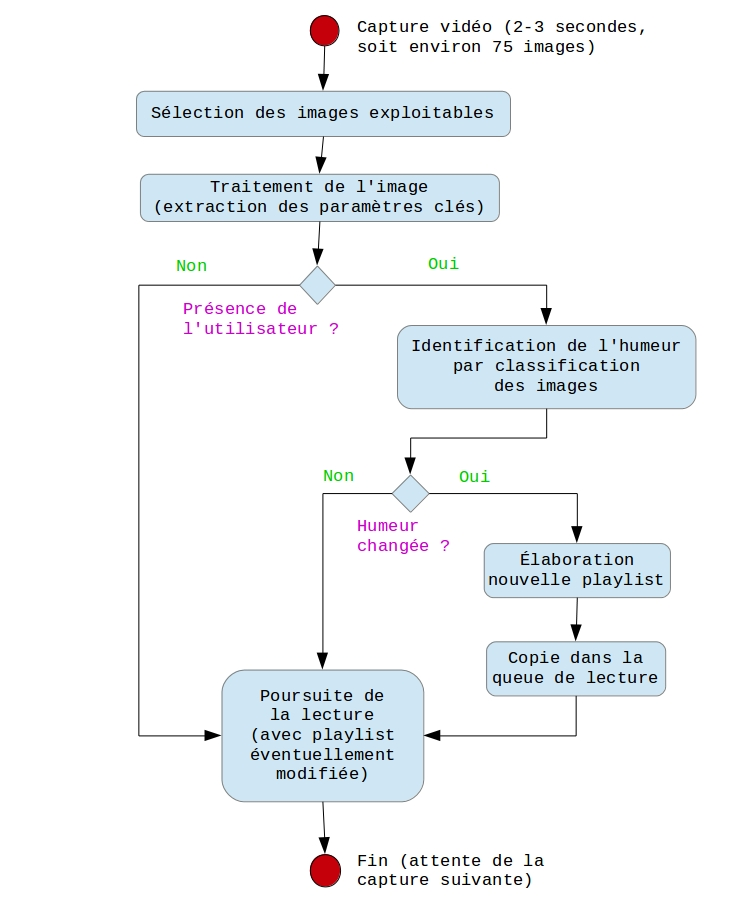
\includegraphics[scale=0.5]{./images/SchemaCaptureVideo2.jpg}
\caption{Opérations effectuées lors d'une capture vidéo par le logiciel dans le cadre d'une utilisation en mode FeelList}
\label{ds1}
\end{figure}

\begin{figure}[htp]
\centering
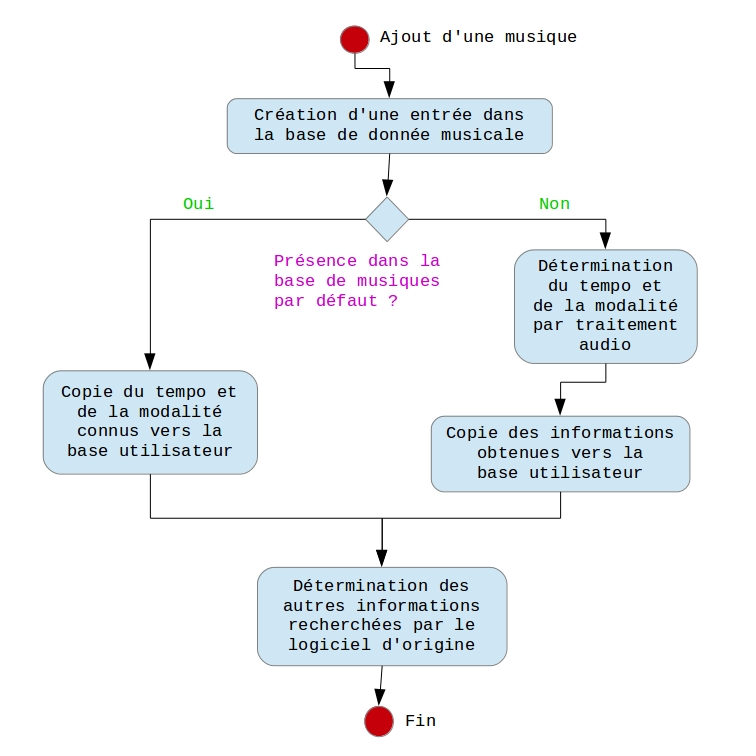
\includegraphics[scale=0.5]{./images/SchemaAjoutMusique2.jpg}
\caption{Opérations effectuées lors de l'ajout d'une musique à la bibliothèque}
\label{ds2}
\end{figure}

\begin{figure}[htp]
\centering
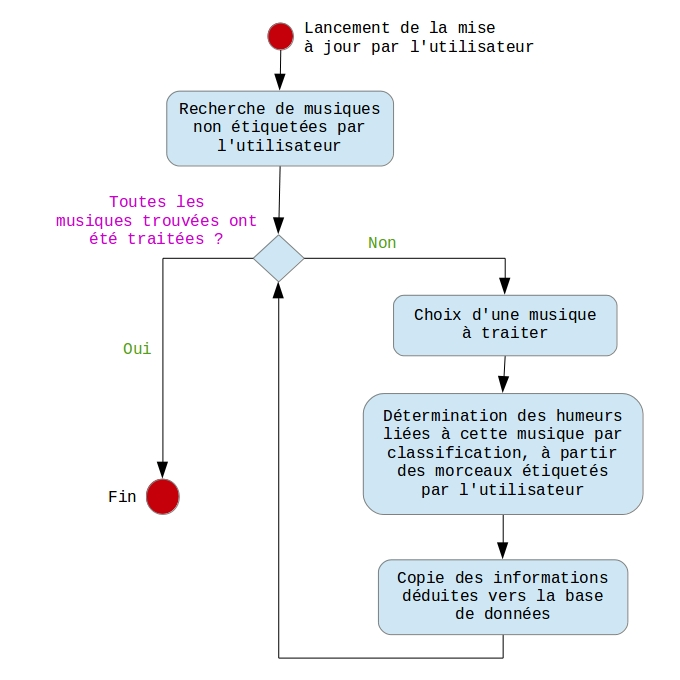
\includegraphics[scale=0.5]{./images/SchemaMiseAJour2.jpg}
\caption{Opérations effectuées lors de le mise à jour de la base de données, avec étiquetage automatique}
\label{ds3}
\end{figure}